\section{深度学习介绍}

\subsection{传统机器学习方法}

在之前的50年左右,传统的模式识别模型用手工定义的特征进行特征提取,通过对数据的分析选取可训分类器进行模型构建。 最近10年,借助现代计算机计算能力的提高和大数据量的爆发,神经网络方法得以重新广泛应用,在很多领域都达到非常好的效果, 我们称这种利用大规模网络进行模式识别方法为深度学习(Deep Learning), 也叫End-To-End Learning。不同于传统模型采用固定特征,或者固定kernel(核函数)进行样本度量; 深度学习采用可训特征(或可训的kernel), 然后将特征作为可训练的分类器输入, 进行训练, 如表\ref{Tab:dl_overview_compare}。

\begin{table}[ht]
\centering
  \begin{tabular}{|c||c|c|c|}
  \hline
   & 特征 & 分类器 & 特点\\
  \hline\hline
   传统方法 & 人工定义的特征 & 简单可训练分类器 & 特征设计费时,需强业务背景\\
  \hline
  深度学习 & 训练特征提取模型 & 复杂可训练分类器 & End-to-End learning,feature易操作\\
  \hline
  \end{tabular}
  \caption{深度学习与传统模式识别方法}
  \centering \label{Tab:dl_overview_compare}
\end{table}

历史上,第一个有学习功能的机器为1960年提出的Perceptron\cite{rosenblatt1960perceptron},也是神经网络的一个基本单元。 Perceptron是一个简单特征提取器上加载的一个线性分类器: 


\begin{equation}
\label{Eq:Perceptron}
y=sign(\sum_{i=1}^N{w_iF_i(x)}+b)
\end{equation}


其中$x$为数据,$F_i(x)$为x的第i个特征,$w_i$为相应的特征权重参数, b为常参数, $sign$为分类器的非线性函数,对于二类分类,$sign$函数将结果映射到(0,1)。

\begin{figure*}[htb]
  \centering
  % Requires \usepackage{graphicx}
  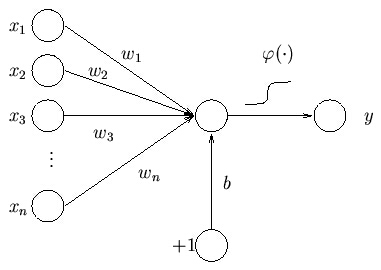
\includegraphics[scale=0.9]{Pictures/CNN/perceptron.jpg}\\
  \caption{Perceptront图例}\label{fig:perceptron}
\end{figure*}

目前最普及的实际应用也用到了线性分类器的一些变种,或者叫模板匹配(template matching)。 但是由于其底层的特征提取器需要反映特定信号的特点, 所以需要由特定领域专家来设置。 比如图像处理领域, 对于不同任务( 图像分类, 图像分割, 图像跟踪等), 所要求的特征就各不相同, 需要针对特定任务定义图像特征。 此外,传统方法也很难设计kernel, 从而不容易表达对距离的度量,仍然以图像来说,最简单的距离度量思路是对应像素相减,但是这显然不能表达图像语义层的相似信息。

为了能使特征更加灵活而且不过多依赖于专家指定的特征, 很多方法提出, 可以先人为定义简单特征, 然后通过无监督学习方法进一步得到中间层特征, 将其输入分类器进行最后分类。
典型的无监督特征学习方法如混合高斯模型\cite{jeong2004image,gray2001gauss,gauvain1992bayesian,reynolds2000speaker,reynolds1995robust, zivkovic2004improved,lee2005effective,yang1999gaussian}, K-Means\cite{liu2007computational,netzer2011reading,coates2011text,dy2004feature,coates2012learning}, 和Sparse Coding\cite{yang2009linear,boureau2008sparse,coates2011importance,coates2011analysis,gao2010local,mairal2010online}。 但这仍然不能解决以下几个问题:

\begin{enumerate}
	\item 建立传统模型代价大\\
	对每个领域,每个任务都需要设计特征。即便有了中间特征层进行无监督的特征选择, 庞大冗余的基础特征的设计也是耗时费力的。 随着工业界对不同任务的需求, 需要建立很多基础特征、 模型, 代价也很大。
	\item 无法很好地利用计算性能\\
	计算机性能的大幅提升本可以用来帮助加速机器学习, 但传统机器学习需要人工定义模型, 从而使模型规模受限,不能很好地利用计算性能和大量数据。 
	
	\item 人工定义特征效果欠佳\\
	目前, 自动学习的特征已经在图像、语音等很多领域强于人工定义的特征。 而且如果需要增加特征维度进行大规模学习就需要再手工定义更多特征, 而不能简单地够自动按比例扩大。
	
\end{enumerate}


\subsection{深度学习方法}

同传统方法的基本思想类似, 深度学习也是从数据分别生成底层特征, 中间层特征, 最后加入高层特征, 输入分类器进行分类。 从图像角度, 如图\ref{fig:feature_level}所示\cite{zeiler2014visualizing,zeiler2013stochastic},图中(a),(b),(c)分别为底层特征,中层特征和高层特征, 其中底层特征学习图像的浅层特征,在所有类别中共享, 如(a)中,学到的特征类似Gabor滤波器所提取的边缘特征\cite{ngiam2010tiled,shi1998gabor}, 从中间层到高层逐渐学习图像的深层语义特征, 如有语义的显著图像区域, 高层特征更为稳定,也具有类属性。  从自然语言处理的角度, 初始输入为字符, 从底层向上依次学习单词, 短语, 长句, 文章。

\begin{figure*}[htb]
  \centering
  % Requires \usepackage{graphicx}
  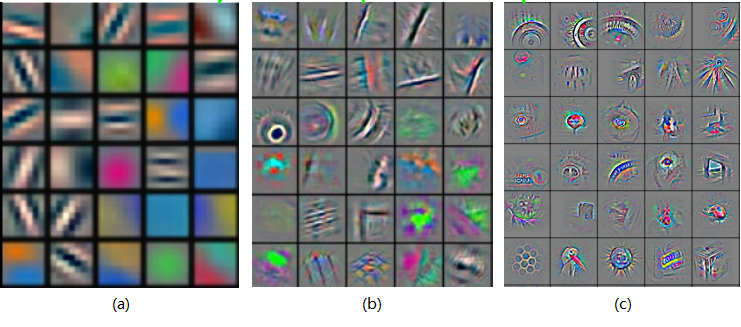
\includegraphics[scale=0.9]{Pictures/CNN/low_mid_high_feature.png}\\
  \caption{各层次feature}\label{fig:feature_level}
\end{figure*}


按训练方法, 神经网络可以分为三类: 
\begin{enumerate}
	\item[有监督学习]
	当样本的标号很全时,我们可以用纯有监督学习方法, 用随机梯度下降算法进行误差反传进行网络训练。 该方法通常用于
\end{enumerate}








